\documentclass[11pt]{article}

    \usepackage[breakable]{tcolorbox}
    \usepackage{parskip} % Stop auto-indenting (to mimic markdown behaviour)
    
    \usepackage{iftex}
    \ifPDFTeX
    	\usepackage[T1]{fontenc}
    	\usepackage{mathpazo}
    \else
    	\usepackage{fontspec}
    \fi

    % Basic figure setup, for now with no caption control since it's done
    % automatically by Pandoc (which extracts ![](path) syntax from Markdown).
    \usepackage{graphicx}
    % Maintain compatibility with old templates. Remove in nbconvert 6.0
    \let\Oldincludegraphics\includegraphics
    % Ensure that by default, figures have no caption (until we provide a
    % proper Figure object with a Caption API and a way to capture that
    % in the conversion process - todo).
    \usepackage{caption}
    \DeclareCaptionFormat{nocaption}{}
    \captionsetup{format=nocaption,aboveskip=0pt,belowskip=0pt}

    \usepackage[Export]{adjustbox} % Used to constrain images to a maximum size
    \adjustboxset{max size={0.9\linewidth}{0.9\paperheight}}
    \usepackage{float}
    \floatplacement{figure}{H} % forces figures to be placed at the correct location
    \usepackage{xcolor} % Allow colors to be defined
    \usepackage{enumerate} % Needed for markdown enumerations to work
    \usepackage{geometry} % Used to adjust the document margins
    \usepackage{amsmath} % Equations
    \usepackage{amssymb} % Equations
    \usepackage{textcomp} % defines textquotesingle
    % Hack from http://tex.stackexchange.com/a/47451/13684:
    \AtBeginDocument{%
        \def\PYZsq{\textquotesingle}% Upright quotes in Pygmentized code
    }
    \usepackage{upquote} % Upright quotes for verbatim code
    \usepackage{eurosym} % defines \euro
    \usepackage[mathletters]{ucs} % Extended unicode (utf-8) support
    \usepackage{fancyvrb} % verbatim replacement that allows latex
    \usepackage{grffile} % extends the file name processing of package graphics 
                         % to support a larger range
    \makeatletter % fix for grffile with XeLaTeX
    \def\Gread@@xetex#1{%
      \IfFileExists{"\Gin@base".bb}%
      {\Gread@eps{\Gin@base.bb}}%
      {\Gread@@xetex@aux#1}%
    }
    \makeatother

    % The hyperref package gives us a pdf with properly built
    % internal navigation ('pdf bookmarks' for the table of contents,
    % internal cross-reference links, web links for URLs, etc.)
    \usepackage{hyperref}
    % The default LaTeX title has an obnoxious amount of whitespace. By default,
    % titling removes some of it. It also provides customization options.
    \usepackage{titling}
    \usepackage{longtable} % longtable support required by pandoc >1.10
    \usepackage{booktabs}  % table support for pandoc > 1.12.2
    \usepackage[inline]{enumitem} % IRkernel/repr support (it uses the enumerate* environment)
    \usepackage[normalem]{ulem} % ulem is needed to support strikethroughs (\sout)
                                % normalem makes italics be italics, not underlines
    \usepackage{mathrsfs}
    

    
    % Colors for the hyperref package
    \definecolor{urlcolor}{rgb}{0,.145,.698}
    \definecolor{linkcolor}{rgb}{.71,0.21,0.01}
    \definecolor{citecolor}{rgb}{.12,.54,.11}

    % ANSI colors
    \definecolor{ansi-black}{HTML}{3E424D}
    \definecolor{ansi-black-intense}{HTML}{282C36}
    \definecolor{ansi-red}{HTML}{E75C58}
    \definecolor{ansi-red-intense}{HTML}{B22B31}
    \definecolor{ansi-green}{HTML}{00A250}
    \definecolor{ansi-green-intense}{HTML}{007427}
    \definecolor{ansi-yellow}{HTML}{DDB62B}
    \definecolor{ansi-yellow-intense}{HTML}{B27D12}
    \definecolor{ansi-blue}{HTML}{208FFB}
    \definecolor{ansi-blue-intense}{HTML}{0065CA}
    \definecolor{ansi-magenta}{HTML}{D160C4}
    \definecolor{ansi-magenta-intense}{HTML}{A03196}
    \definecolor{ansi-cyan}{HTML}{60C6C8}
    \definecolor{ansi-cyan-intense}{HTML}{258F8F}
    \definecolor{ansi-white}{HTML}{C5C1B4}
    \definecolor{ansi-white-intense}{HTML}{A1A6B2}
    \definecolor{ansi-default-inverse-fg}{HTML}{FFFFFF}
    \definecolor{ansi-default-inverse-bg}{HTML}{000000}

    % commands and environments needed by pandoc snippets
    % extracted from the output of `pandoc -s`
    \providecommand{\tightlist}{%
      \setlength{\itemsep}{0pt}\setlength{\parskip}{0pt}}
    \DefineVerbatimEnvironment{Highlighting}{Verbatim}{commandchars=\\\{\}}
    % Add ',fontsize=\small' for more characters per line
    \newenvironment{Shaded}{}{}
    \newcommand{\KeywordTok}[1]{\textcolor[rgb]{0.00,0.44,0.13}{\textbf{{#1}}}}
    \newcommand{\DataTypeTok}[1]{\textcolor[rgb]{0.56,0.13,0.00}{{#1}}}
    \newcommand{\DecValTok}[1]{\textcolor[rgb]{0.25,0.63,0.44}{{#1}}}
    \newcommand{\BaseNTok}[1]{\textcolor[rgb]{0.25,0.63,0.44}{{#1}}}
    \newcommand{\FloatTok}[1]{\textcolor[rgb]{0.25,0.63,0.44}{{#1}}}
    \newcommand{\CharTok}[1]{\textcolor[rgb]{0.25,0.44,0.63}{{#1}}}
    \newcommand{\StringTok}[1]{\textcolor[rgb]{0.25,0.44,0.63}{{#1}}}
    \newcommand{\CommentTok}[1]{\textcolor[rgb]{0.38,0.63,0.69}{\textit{{#1}}}}
    \newcommand{\OtherTok}[1]{\textcolor[rgb]{0.00,0.44,0.13}{{#1}}}
    \newcommand{\AlertTok}[1]{\textcolor[rgb]{1.00,0.00,0.00}{\textbf{{#1}}}}
    \newcommand{\FunctionTok}[1]{\textcolor[rgb]{0.02,0.16,0.49}{{#1}}}
    \newcommand{\RegionMarkerTok}[1]{{#1}}
    \newcommand{\ErrorTok}[1]{\textcolor[rgb]{1.00,0.00,0.00}{\textbf{{#1}}}}
    \newcommand{\NormalTok}[1]{{#1}}
    
    % Additional commands for more recent versions of Pandoc
    \newcommand{\ConstantTok}[1]{\textcolor[rgb]{0.53,0.00,0.00}{{#1}}}
    \newcommand{\SpecialCharTok}[1]{\textcolor[rgb]{0.25,0.44,0.63}{{#1}}}
    \newcommand{\VerbatimStringTok}[1]{\textcolor[rgb]{0.25,0.44,0.63}{{#1}}}
    \newcommand{\SpecialStringTok}[1]{\textcolor[rgb]{0.73,0.40,0.53}{{#1}}}
    \newcommand{\ImportTok}[1]{{#1}}
    \newcommand{\DocumentationTok}[1]{\textcolor[rgb]{0.73,0.13,0.13}{\textit{{#1}}}}
    \newcommand{\AnnotationTok}[1]{\textcolor[rgb]{0.38,0.63,0.69}{\textbf{\textit{{#1}}}}}
    \newcommand{\CommentVarTok}[1]{\textcolor[rgb]{0.38,0.63,0.69}{\textbf{\textit{{#1}}}}}
    \newcommand{\VariableTok}[1]{\textcolor[rgb]{0.10,0.09,0.49}{{#1}}}
    \newcommand{\ControlFlowTok}[1]{\textcolor[rgb]{0.00,0.44,0.13}{\textbf{{#1}}}}
    \newcommand{\OperatorTok}[1]{\textcolor[rgb]{0.40,0.40,0.40}{{#1}}}
    \newcommand{\BuiltInTok}[1]{{#1}}
    \newcommand{\ExtensionTok}[1]{{#1}}
    \newcommand{\PreprocessorTok}[1]{\textcolor[rgb]{0.74,0.48,0.00}{{#1}}}
    \newcommand{\AttributeTok}[1]{\textcolor[rgb]{0.49,0.56,0.16}{{#1}}}
    \newcommand{\InformationTok}[1]{\textcolor[rgb]{0.38,0.63,0.69}{\textbf{\textit{{#1}}}}}
    \newcommand{\WarningTok}[1]{\textcolor[rgb]{0.38,0.63,0.69}{\textbf{\textit{{#1}}}}}
    
    
    % Define a nice break command that doesn't care if a line doesn't already
    % exist.
    \def\br{\hspace*{\fill} \\* }
    % Math Jax compatibility definitions
    \def\gt{>}
    \def\lt{<}
    \let\Oldtex\TeX
    \let\Oldlatex\LaTeX
    \renewcommand{\TeX}{\textrm{\Oldtex}}
    \renewcommand{\LaTeX}{\textrm{\Oldlatex}}
    % Document parameters
    % Document title
    \title{Comparing numerical results with experimental data}
    
    
    
    
    
% Pygments definitions
\makeatletter
\def\PY@reset{\let\PY@it=\relax \let\PY@bf=\relax%
    \let\PY@ul=\relax \let\PY@tc=\relax%
    \let\PY@bc=\relax \let\PY@ff=\relax}
\def\PY@tok#1{\csname PY@tok@#1\endcsname}
\def\PY@toks#1+{\ifx\relax#1\empty\else%
    \PY@tok{#1}\expandafter\PY@toks\fi}
\def\PY@do#1{\PY@bc{\PY@tc{\PY@ul{%
    \PY@it{\PY@bf{\PY@ff{#1}}}}}}}
\def\PY#1#2{\PY@reset\PY@toks#1+\relax+\PY@do{#2}}

\expandafter\def\csname PY@tok@w\endcsname{\def\PY@tc##1{\textcolor[rgb]{0.73,0.73,0.73}{##1}}}
\expandafter\def\csname PY@tok@c\endcsname{\let\PY@it=\textit\def\PY@tc##1{\textcolor[rgb]{0.25,0.50,0.50}{##1}}}
\expandafter\def\csname PY@tok@cp\endcsname{\def\PY@tc##1{\textcolor[rgb]{0.74,0.48,0.00}{##1}}}
\expandafter\def\csname PY@tok@k\endcsname{\let\PY@bf=\textbf\def\PY@tc##1{\textcolor[rgb]{0.00,0.50,0.00}{##1}}}
\expandafter\def\csname PY@tok@kp\endcsname{\def\PY@tc##1{\textcolor[rgb]{0.00,0.50,0.00}{##1}}}
\expandafter\def\csname PY@tok@kt\endcsname{\def\PY@tc##1{\textcolor[rgb]{0.69,0.00,0.25}{##1}}}
\expandafter\def\csname PY@tok@o\endcsname{\def\PY@tc##1{\textcolor[rgb]{0.40,0.40,0.40}{##1}}}
\expandafter\def\csname PY@tok@ow\endcsname{\let\PY@bf=\textbf\def\PY@tc##1{\textcolor[rgb]{0.67,0.13,1.00}{##1}}}
\expandafter\def\csname PY@tok@nb\endcsname{\def\PY@tc##1{\textcolor[rgb]{0.00,0.50,0.00}{##1}}}
\expandafter\def\csname PY@tok@nf\endcsname{\def\PY@tc##1{\textcolor[rgb]{0.00,0.00,1.00}{##1}}}
\expandafter\def\csname PY@tok@nc\endcsname{\let\PY@bf=\textbf\def\PY@tc##1{\textcolor[rgb]{0.00,0.00,1.00}{##1}}}
\expandafter\def\csname PY@tok@nn\endcsname{\let\PY@bf=\textbf\def\PY@tc##1{\textcolor[rgb]{0.00,0.00,1.00}{##1}}}
\expandafter\def\csname PY@tok@ne\endcsname{\let\PY@bf=\textbf\def\PY@tc##1{\textcolor[rgb]{0.82,0.25,0.23}{##1}}}
\expandafter\def\csname PY@tok@nv\endcsname{\def\PY@tc##1{\textcolor[rgb]{0.10,0.09,0.49}{##1}}}
\expandafter\def\csname PY@tok@no\endcsname{\def\PY@tc##1{\textcolor[rgb]{0.53,0.00,0.00}{##1}}}
\expandafter\def\csname PY@tok@nl\endcsname{\def\PY@tc##1{\textcolor[rgb]{0.63,0.63,0.00}{##1}}}
\expandafter\def\csname PY@tok@ni\endcsname{\let\PY@bf=\textbf\def\PY@tc##1{\textcolor[rgb]{0.60,0.60,0.60}{##1}}}
\expandafter\def\csname PY@tok@na\endcsname{\def\PY@tc##1{\textcolor[rgb]{0.49,0.56,0.16}{##1}}}
\expandafter\def\csname PY@tok@nt\endcsname{\let\PY@bf=\textbf\def\PY@tc##1{\textcolor[rgb]{0.00,0.50,0.00}{##1}}}
\expandafter\def\csname PY@tok@nd\endcsname{\def\PY@tc##1{\textcolor[rgb]{0.67,0.13,1.00}{##1}}}
\expandafter\def\csname PY@tok@s\endcsname{\def\PY@tc##1{\textcolor[rgb]{0.73,0.13,0.13}{##1}}}
\expandafter\def\csname PY@tok@sd\endcsname{\let\PY@it=\textit\def\PY@tc##1{\textcolor[rgb]{0.73,0.13,0.13}{##1}}}
\expandafter\def\csname PY@tok@si\endcsname{\let\PY@bf=\textbf\def\PY@tc##1{\textcolor[rgb]{0.73,0.40,0.53}{##1}}}
\expandafter\def\csname PY@tok@se\endcsname{\let\PY@bf=\textbf\def\PY@tc##1{\textcolor[rgb]{0.73,0.40,0.13}{##1}}}
\expandafter\def\csname PY@tok@sr\endcsname{\def\PY@tc##1{\textcolor[rgb]{0.73,0.40,0.53}{##1}}}
\expandafter\def\csname PY@tok@ss\endcsname{\def\PY@tc##1{\textcolor[rgb]{0.10,0.09,0.49}{##1}}}
\expandafter\def\csname PY@tok@sx\endcsname{\def\PY@tc##1{\textcolor[rgb]{0.00,0.50,0.00}{##1}}}
\expandafter\def\csname PY@tok@m\endcsname{\def\PY@tc##1{\textcolor[rgb]{0.40,0.40,0.40}{##1}}}
\expandafter\def\csname PY@tok@gh\endcsname{\let\PY@bf=\textbf\def\PY@tc##1{\textcolor[rgb]{0.00,0.00,0.50}{##1}}}
\expandafter\def\csname PY@tok@gu\endcsname{\let\PY@bf=\textbf\def\PY@tc##1{\textcolor[rgb]{0.50,0.00,0.50}{##1}}}
\expandafter\def\csname PY@tok@gd\endcsname{\def\PY@tc##1{\textcolor[rgb]{0.63,0.00,0.00}{##1}}}
\expandafter\def\csname PY@tok@gi\endcsname{\def\PY@tc##1{\textcolor[rgb]{0.00,0.63,0.00}{##1}}}
\expandafter\def\csname PY@tok@gr\endcsname{\def\PY@tc##1{\textcolor[rgb]{1.00,0.00,0.00}{##1}}}
\expandafter\def\csname PY@tok@ge\endcsname{\let\PY@it=\textit}
\expandafter\def\csname PY@tok@gs\endcsname{\let\PY@bf=\textbf}
\expandafter\def\csname PY@tok@gp\endcsname{\let\PY@bf=\textbf\def\PY@tc##1{\textcolor[rgb]{0.00,0.00,0.50}{##1}}}
\expandafter\def\csname PY@tok@go\endcsname{\def\PY@tc##1{\textcolor[rgb]{0.53,0.53,0.53}{##1}}}
\expandafter\def\csname PY@tok@gt\endcsname{\def\PY@tc##1{\textcolor[rgb]{0.00,0.27,0.87}{##1}}}
\expandafter\def\csname PY@tok@err\endcsname{\def\PY@bc##1{\setlength{\fboxsep}{0pt}\fcolorbox[rgb]{1.00,0.00,0.00}{1,1,1}{\strut ##1}}}
\expandafter\def\csname PY@tok@kc\endcsname{\let\PY@bf=\textbf\def\PY@tc##1{\textcolor[rgb]{0.00,0.50,0.00}{##1}}}
\expandafter\def\csname PY@tok@kd\endcsname{\let\PY@bf=\textbf\def\PY@tc##1{\textcolor[rgb]{0.00,0.50,0.00}{##1}}}
\expandafter\def\csname PY@tok@kn\endcsname{\let\PY@bf=\textbf\def\PY@tc##1{\textcolor[rgb]{0.00,0.50,0.00}{##1}}}
\expandafter\def\csname PY@tok@kr\endcsname{\let\PY@bf=\textbf\def\PY@tc##1{\textcolor[rgb]{0.00,0.50,0.00}{##1}}}
\expandafter\def\csname PY@tok@bp\endcsname{\def\PY@tc##1{\textcolor[rgb]{0.00,0.50,0.00}{##1}}}
\expandafter\def\csname PY@tok@fm\endcsname{\def\PY@tc##1{\textcolor[rgb]{0.00,0.00,1.00}{##1}}}
\expandafter\def\csname PY@tok@vc\endcsname{\def\PY@tc##1{\textcolor[rgb]{0.10,0.09,0.49}{##1}}}
\expandafter\def\csname PY@tok@vg\endcsname{\def\PY@tc##1{\textcolor[rgb]{0.10,0.09,0.49}{##1}}}
\expandafter\def\csname PY@tok@vi\endcsname{\def\PY@tc##1{\textcolor[rgb]{0.10,0.09,0.49}{##1}}}
\expandafter\def\csname PY@tok@vm\endcsname{\def\PY@tc##1{\textcolor[rgb]{0.10,0.09,0.49}{##1}}}
\expandafter\def\csname PY@tok@sa\endcsname{\def\PY@tc##1{\textcolor[rgb]{0.73,0.13,0.13}{##1}}}
\expandafter\def\csname PY@tok@sb\endcsname{\def\PY@tc##1{\textcolor[rgb]{0.73,0.13,0.13}{##1}}}
\expandafter\def\csname PY@tok@sc\endcsname{\def\PY@tc##1{\textcolor[rgb]{0.73,0.13,0.13}{##1}}}
\expandafter\def\csname PY@tok@dl\endcsname{\def\PY@tc##1{\textcolor[rgb]{0.73,0.13,0.13}{##1}}}
\expandafter\def\csname PY@tok@s2\endcsname{\def\PY@tc##1{\textcolor[rgb]{0.73,0.13,0.13}{##1}}}
\expandafter\def\csname PY@tok@sh\endcsname{\def\PY@tc##1{\textcolor[rgb]{0.73,0.13,0.13}{##1}}}
\expandafter\def\csname PY@tok@s1\endcsname{\def\PY@tc##1{\textcolor[rgb]{0.73,0.13,0.13}{##1}}}
\expandafter\def\csname PY@tok@mb\endcsname{\def\PY@tc##1{\textcolor[rgb]{0.40,0.40,0.40}{##1}}}
\expandafter\def\csname PY@tok@mf\endcsname{\def\PY@tc##1{\textcolor[rgb]{0.40,0.40,0.40}{##1}}}
\expandafter\def\csname PY@tok@mh\endcsname{\def\PY@tc##1{\textcolor[rgb]{0.40,0.40,0.40}{##1}}}
\expandafter\def\csname PY@tok@mi\endcsname{\def\PY@tc##1{\textcolor[rgb]{0.40,0.40,0.40}{##1}}}
\expandafter\def\csname PY@tok@il\endcsname{\def\PY@tc##1{\textcolor[rgb]{0.40,0.40,0.40}{##1}}}
\expandafter\def\csname PY@tok@mo\endcsname{\def\PY@tc##1{\textcolor[rgb]{0.40,0.40,0.40}{##1}}}
\expandafter\def\csname PY@tok@ch\endcsname{\let\PY@it=\textit\def\PY@tc##1{\textcolor[rgb]{0.25,0.50,0.50}{##1}}}
\expandafter\def\csname PY@tok@cm\endcsname{\let\PY@it=\textit\def\PY@tc##1{\textcolor[rgb]{0.25,0.50,0.50}{##1}}}
\expandafter\def\csname PY@tok@cpf\endcsname{\let\PY@it=\textit\def\PY@tc##1{\textcolor[rgb]{0.25,0.50,0.50}{##1}}}
\expandafter\def\csname PY@tok@c1\endcsname{\let\PY@it=\textit\def\PY@tc##1{\textcolor[rgb]{0.25,0.50,0.50}{##1}}}
\expandafter\def\csname PY@tok@cs\endcsname{\let\PY@it=\textit\def\PY@tc##1{\textcolor[rgb]{0.25,0.50,0.50}{##1}}}

\def\PYZbs{\char`\\}
\def\PYZus{\char`\_}
\def\PYZob{\char`\{}
\def\PYZcb{\char`\}}
\def\PYZca{\char`\^}
\def\PYZam{\char`\&}
\def\PYZlt{\char`\<}
\def\PYZgt{\char`\>}
\def\PYZsh{\char`\#}
\def\PYZpc{\char`\%}
\def\PYZdl{\char`\$}
\def\PYZhy{\char`\-}
\def\PYZsq{\char`\'}
\def\PYZdq{\char`\"}
\def\PYZti{\char`\~}
% for compatibility with earlier versions
\def\PYZat{@}
\def\PYZlb{[}
\def\PYZrb{]}
\makeatother


    % For linebreaks inside Verbatim environment from package fancyvrb. 
    \makeatletter
        \newbox\Wrappedcontinuationbox 
        \newbox\Wrappedvisiblespacebox 
        \newcommand*\Wrappedvisiblespace {\textcolor{red}{\textvisiblespace}} 
        \newcommand*\Wrappedcontinuationsymbol {\textcolor{red}{\llap{\tiny$\m@th\hookrightarrow$}}} 
        \newcommand*\Wrappedcontinuationindent {3ex } 
        \newcommand*\Wrappedafterbreak {\kern\Wrappedcontinuationindent\copy\Wrappedcontinuationbox} 
        % Take advantage of the already applied Pygments mark-up to insert 
        % potential linebreaks for TeX processing. 
        %        {, <, #, %, $, ' and ": go to next line. 
        %        _, }, ^, &, >, - and ~: stay at end of broken line. 
        % Use of \textquotesingle for straight quote. 
        \newcommand*\Wrappedbreaksatspecials {% 
            \def\PYGZus{\discretionary{\char`\_}{\Wrappedafterbreak}{\char`\_}}% 
            \def\PYGZob{\discretionary{}{\Wrappedafterbreak\char`\{}{\char`\{}}% 
            \def\PYGZcb{\discretionary{\char`\}}{\Wrappedafterbreak}{\char`\}}}% 
            \def\PYGZca{\discretionary{\char`\^}{\Wrappedafterbreak}{\char`\^}}% 
            \def\PYGZam{\discretionary{\char`\&}{\Wrappedafterbreak}{\char`\&}}% 
            \def\PYGZlt{\discretionary{}{\Wrappedafterbreak\char`\<}{\char`\<}}% 
            \def\PYGZgt{\discretionary{\char`\>}{\Wrappedafterbreak}{\char`\>}}% 
            \def\PYGZsh{\discretionary{}{\Wrappedafterbreak\char`\#}{\char`\#}}% 
            \def\PYGZpc{\discretionary{}{\Wrappedafterbreak\char`\%}{\char`\%}}% 
            \def\PYGZdl{\discretionary{}{\Wrappedafterbreak\char`\$}{\char`\$}}% 
            \def\PYGZhy{\discretionary{\char`\-}{\Wrappedafterbreak}{\char`\-}}% 
            \def\PYGZsq{\discretionary{}{\Wrappedafterbreak\textquotesingle}{\textquotesingle}}% 
            \def\PYGZdq{\discretionary{}{\Wrappedafterbreak\char`\"}{\char`\"}}% 
            \def\PYGZti{\discretionary{\char`\~}{\Wrappedafterbreak}{\char`\~}}% 
        } 
        % Some characters . , ; ? ! / are not pygmentized. 
        % This macro makes them "active" and they will insert potential linebreaks 
        \newcommand*\Wrappedbreaksatpunct {% 
            \lccode`\~`\.\lowercase{\def~}{\discretionary{\hbox{\char`\.}}{\Wrappedafterbreak}{\hbox{\char`\.}}}% 
            \lccode`\~`\,\lowercase{\def~}{\discretionary{\hbox{\char`\,}}{\Wrappedafterbreak}{\hbox{\char`\,}}}% 
            \lccode`\~`\;\lowercase{\def~}{\discretionary{\hbox{\char`\;}}{\Wrappedafterbreak}{\hbox{\char`\;}}}% 
            \lccode`\~`\:\lowercase{\def~}{\discretionary{\hbox{\char`\:}}{\Wrappedafterbreak}{\hbox{\char`\:}}}% 
            \lccode`\~`\?\lowercase{\def~}{\discretionary{\hbox{\char`\?}}{\Wrappedafterbreak}{\hbox{\char`\?}}}% 
            \lccode`\~`\!\lowercase{\def~}{\discretionary{\hbox{\char`\!}}{\Wrappedafterbreak}{\hbox{\char`\!}}}% 
            \lccode`\~`\/\lowercase{\def~}{\discretionary{\hbox{\char`\/}}{\Wrappedafterbreak}{\hbox{\char`\/}}}% 
            \catcode`\.\active
            \catcode`\,\active 
            \catcode`\;\active
            \catcode`\:\active
            \catcode`\?\active
            \catcode`\!\active
            \catcode`\/\active 
            \lccode`\~`\~ 	
        }
    \makeatother

    \let\OriginalVerbatim=\Verbatim
    \makeatletter
    \renewcommand{\Verbatim}[1][1]{%
        %\parskip\z@skip
        \sbox\Wrappedcontinuationbox {\Wrappedcontinuationsymbol}%
        \sbox\Wrappedvisiblespacebox {\FV@SetupFont\Wrappedvisiblespace}%
        \def\FancyVerbFormatLine ##1{\hsize\linewidth
            \vtop{\raggedright\hyphenpenalty\z@\exhyphenpenalty\z@
                \doublehyphendemerits\z@\finalhyphendemerits\z@
                \strut ##1\strut}%
        }%
        % If the linebreak is at a space, the latter will be displayed as visible
        % space at end of first line, and a continuation symbol starts next line.
        % Stretch/shrink are however usually zero for typewriter font.
        \def\FV@Space {%
            \nobreak\hskip\z@ plus\fontdimen3\font minus\fontdimen4\font
            \discretionary{\copy\Wrappedvisiblespacebox}{\Wrappedafterbreak}
            {\kern\fontdimen2\font}%
        }%
        
        % Allow breaks at special characters using \PYG... macros.
        \Wrappedbreaksatspecials
        % Breaks at punctuation characters . , ; ? ! and / need catcode=\active 	
        \OriginalVerbatim[#1,codes*=\Wrappedbreaksatpunct]%
    }
    \makeatother

    % Exact colors from NB
    \definecolor{incolor}{HTML}{303F9F}
    \definecolor{outcolor}{HTML}{D84315}
    \definecolor{cellborder}{HTML}{CFCFCF}
    \definecolor{cellbackground}{HTML}{F7F7F7}
    
    % prompt
    \makeatletter
    \newcommand{\boxspacing}{\kern\kvtcb@left@rule\kern\kvtcb@boxsep}
    \makeatother
    \newcommand{\prompt}[4]{
        \ttfamily\llap{{\color{#2}[#3]:\hspace{3pt}#4}}\vspace{-\baselineskip}
    }
    

    
    % Prevent overflowing lines due to hard-to-break entities
    \sloppy 
    % Setup hyperref package
    \hypersetup{
      breaklinks=true,  % so long urls are correctly broken across lines
      colorlinks=true,
      urlcolor=urlcolor,
      linkcolor=linkcolor,
      citecolor=citecolor,
      }
    % Slightly bigger margins than the latex defaults
    
    \geometry{verbose,tmargin=1in,bmargin=1in,lmargin=1in,rmargin=1in}
    
    

\begin{document}
    
    \maketitle
    
    

    
    \setcounter{page}{87}
\tableofcontents 
\setcounter{section}{0}

    \hypertarget{abstract}{%
\section{Abstract}\label{abstract}}

Experimental data from simultaneous work function and resistance
measurements will be compared with the results from the numerical
calculations. Results from an \(SnO_2\) gas sensor measured at 300°C
will be used to demonstrate, how numerical data can be used to gain more
insights about the measured material. The chosen dataset the the
graphical representation originates from the Phd. thesis of Julia
Rebholz: \cite{Rebholz2016a}.

The data was generated by exposing the sensor to various gas
compositions of \(H_2\), \(CO\), \(O_2\) and \(N_2\). The surface
potential changes \(\Delta V\) resulting from the different gas
atmosphere have been obtained with the Kelvin probe technique.
Simultaneously the corresponding resistance was measured. The data point
point at \(0e\Delta V\) corresponds to the situation in nitrogen.

These experimental data points will be compared with the results
obtained from the numerical model.

    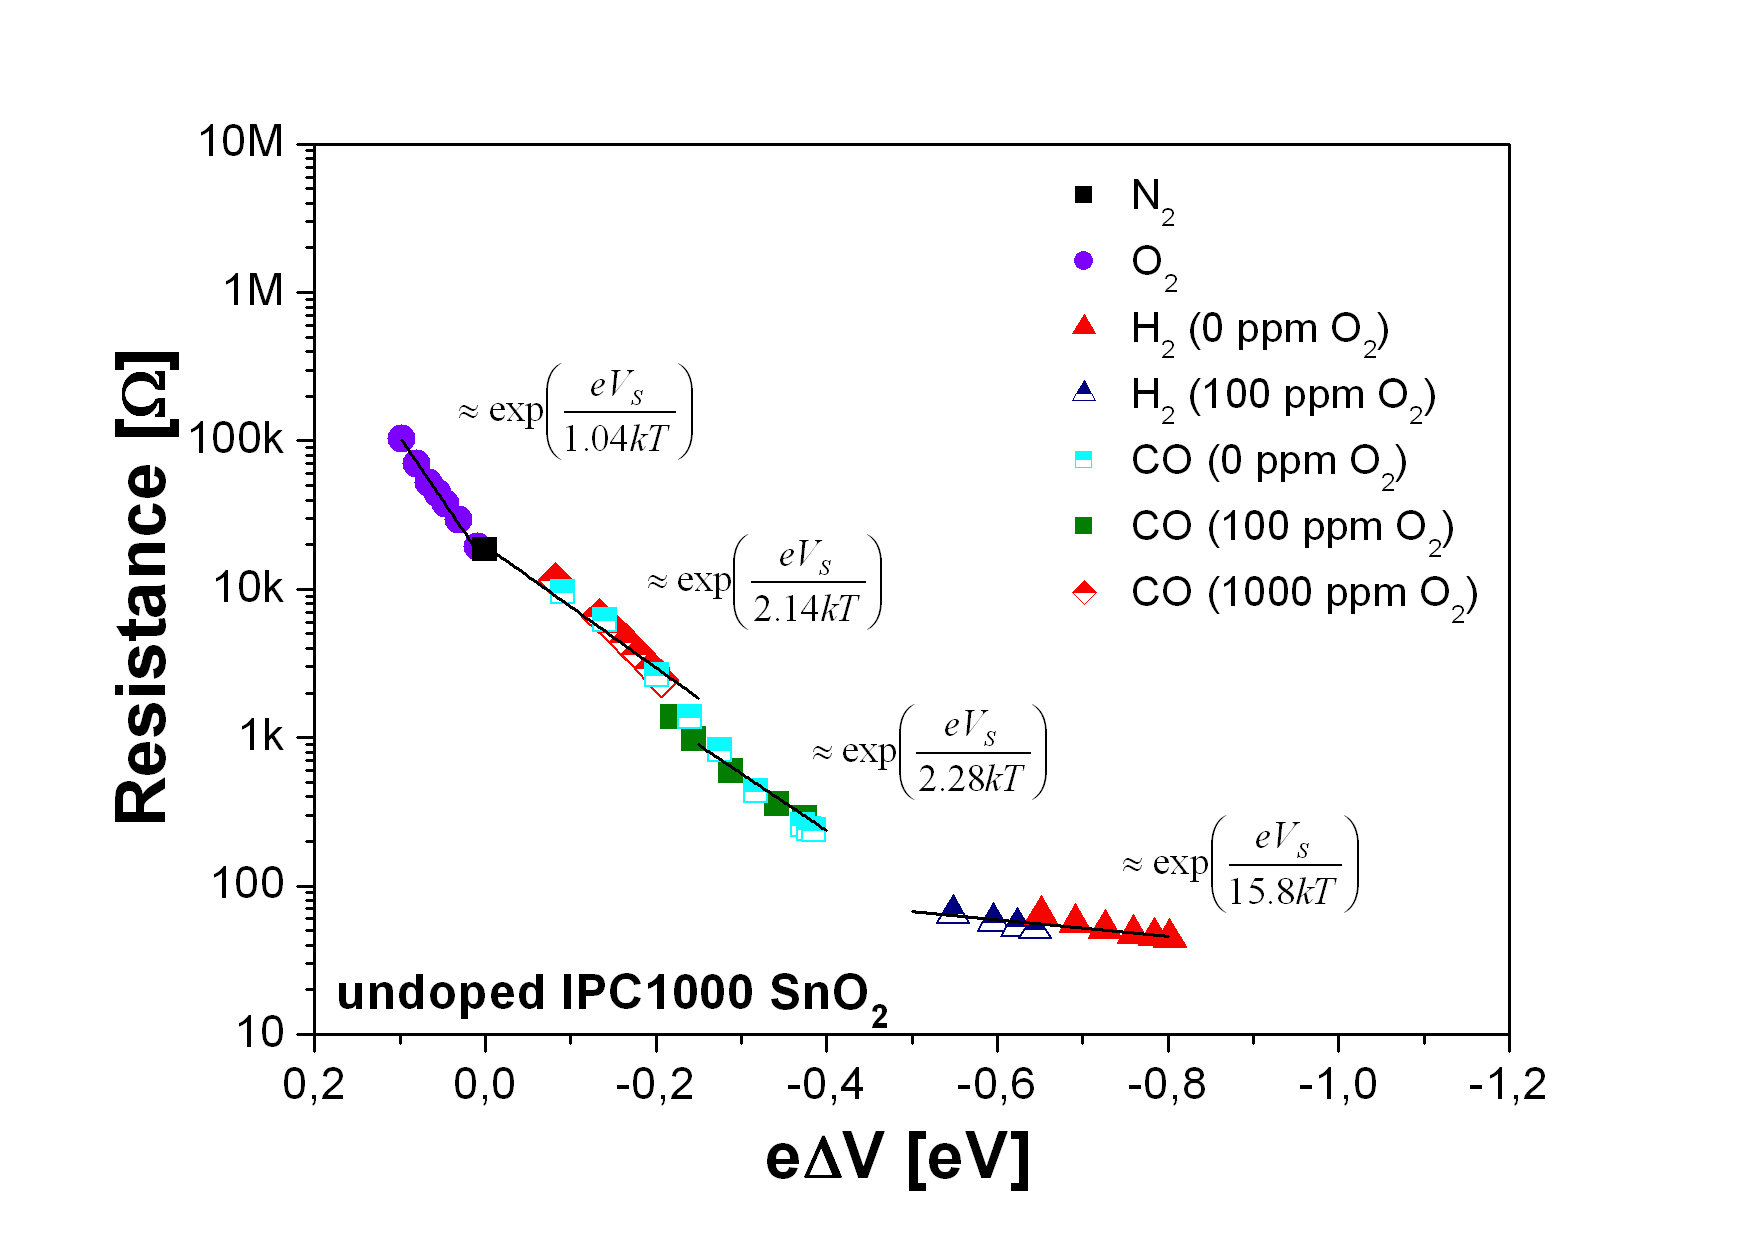
\includegraphics{media/IPC1000undoped_RgegqdV.JPG}

    \hypertarget{fitting-experimental-data-to-numerical-results}{%
\section{Fitting experimental data to numerical
results}\label{fitting-experimental-data-to-numerical-results}}

\hypertarget{importing-experimental-and-numerical-data}{%
\subsection{Importing experimental and numerical
data}\label{importing-experimental-and-numerical-data}}

The data is saved in an excel file, which will be loaded by using the
tools provided by \texttt{pandas}.

    \begin{tcolorbox}[breakable, size=fbox, boxrule=1pt, pad at break*=1mm,colback=cellbackground, colframe=cellborder]
\prompt{In}{incolor}{43}{\boxspacing}
\begin{Verbatim}[commandchars=\\\{\}]
\PY{c+c1}{\PYZsh{}Setting up the env.}
\PY{k+kn}{from} \PY{n+nn}{part2} \PY{k+kn}{import} \PY{o}{*}
\PY{k+kn}{import} \PY{n+nn}{pandas} \PY{k}{as} \PY{n+nn}{pd}
\PY{o}{\PYZpc{}}\PY{k}{pylab} inline

\PY{c+c1}{\PYZsh{}importing the data}
\PY{n}{calc\PYZus{}dF} \PY{o}{=} \PY{n}{pd}\PY{o}{.}\PY{n}{read\PYZus{}hdf}\PY{p}{(}\PY{l+s+s1}{\PYZsq{}}\PY{l+s+s1}{numerical\PYZus{}sol.h5}\PY{l+s+s1}{\PYZsq{}}\PY{p}{,}\PY{l+s+s1}{\PYZsq{}}\PY{l+s+s1}{raw}\PY{l+s+s1}{\PYZsq{}}\PY{p}{)}
\PY{n}{dF\PYZus{}1000} \PY{o}{=} \PY{n}{pd}\PY{o}{.}\PY{n}{read\PYZus{}excel}\PY{p}{(}\PY{l+s+s1}{\PYZsq{}}\PY{l+s+s1}{Kelvin\PYZus{}Data.xlsx}\PY{l+s+s1}{\PYZsq{}}\PY{p}{,} \PY{n}{sheet\PYZus{}name}\PY{o}{=}\PY{l+s+s1}{\PYZsq{}}\PY{l+s+s1}{ipc1000}\PY{l+s+s1}{\PYZsq{}}\PY{p}{)}\PY{o}{.}\PY{n}{sort\PYZus{}values}\PY{p}{(}\PY{n}{by}\PY{o}{=}\PY{l+s+s1}{\PYZsq{}}\PY{l+s+s1}{dV}\PY{l+s+s1}{\PYZsq{}}\PY{p}{)}

\PY{c+c1}{\PYZsh{}instead of unsing the row number}
\PY{c+c1}{\PYZsh{}each row has the value of dV as index}
\PY{n}{dF\PYZus{}1000}\PY{o}{.}\PY{n}{index} \PY{o}{=} \PY{n}{dF\PYZus{}1000}\PY{p}{[}\PY{l+s+s1}{\PYZsq{}}\PY{l+s+s1}{dV}\PY{l+s+s1}{\PYZsq{}}\PY{p}{]}
\end{Verbatim}
\end{tcolorbox}

    \begin{Verbatim}[commandchars=\\\{\}]
Populating the interactive namespace from numpy and matplotlib
    \end{Verbatim}

    \hypertarget{representing-the-raw-data}{%
\subsection{Representing the raw data}\label{representing-the-raw-data}}

    \begin{tcolorbox}[breakable, size=fbox, boxrule=1pt, pad at break*=1mm,colback=cellbackground, colframe=cellborder]
\prompt{In}{incolor}{47}{\boxspacing}
\begin{Verbatim}[commandchars=\\\{\}]
\PY{k}{def} \PY{n+nf}{format\PYZus{}axe}\PY{p}{(}\PY{n}{axe}\PY{p}{,} \PY{n}{ylabel} \PY{o}{=} \PY{k+kc}{None}\PY{p}{,} \PY{n}{set\PYZus{}ylim}\PY{o}{=}\PY{k+kc}{False}\PY{p}{)}\PY{p}{:}
    \PY{n}{labelsize} \PY{o}{=} \PY{l+m+mi}{30}
    \PY{k}{if} \PY{n}{set\PYZus{}ylim}\PY{p}{:}
        \PY{n}{axe}\PY{o}{.}\PY{n}{set\PYZus{}ylim}\PY{p}{(}\PY{p}{(}\PY{l+m+mf}{1e\PYZhy{}4}\PY{p}{,}\PY{l+m+mf}{1e3}\PY{p}{)}\PY{p}{)}
    \PY{n}{axe}\PY{o}{.}\PY{n}{set\PYZus{}yscale}\PY{p}{(}\PY{l+s+s1}{\PYZsq{}}\PY{l+s+s1}{log}\PY{l+s+s1}{\PYZsq{}}\PY{p}{)}
    \PY{n}{axe}\PY{o}{.}\PY{n}{set\PYZus{}xlim}\PY{p}{(}\PY{p}{(}\PY{l+m+mf}{0.2}\PY{p}{,}\PY{o}{\PYZhy{}}\PY{l+m+mf}{1.2}\PY{p}{)}\PY{p}{)}
    \PY{k}{if} \PY{n}{ylabel}\PY{p}{:}
        \PY{n}{axe}\PY{o}{.}\PY{n}{set\PYZus{}ylabel}\PY{p}{(}\PY{n}{ylabel}\PY{p}{,} \PY{n}{fontsize} \PY{o}{=} \PY{n}{labelsize}\PY{p}{)}
    \PY{k}{else}\PY{p}{:}
        \PY{n}{axe}\PY{o}{.}\PY{n}{set\PYZus{}ylabel}\PY{p}{(}\PY{l+s+sa}{r}\PY{l+s+s1}{\PYZsq{}}\PY{l+s+s1}{\PYZdl{}}\PY{l+s+s1}{\PYZbs{}}\PY{l+s+s1}{frac}\PY{l+s+s1}{\PYZob{}}\PY{l+s+s1}{R\PYZus{}}\PY{l+s+si}{\PYZob{}V\PYZus{}S\PYZcb{}}\PY{l+s+s1}{\PYZcb{}}\PY{l+s+s1}{\PYZob{}}\PY{l+s+s1}{R\PYZus{}}\PY{l+s+s1}{\PYZob{}}\PY{l+s+s1}{(V\PYZus{}S=0)\PYZcb{}\PYZcb{}\PYZdl{}}\PY{l+s+s1}{\PYZsq{}}\PY{p}{,} \PY{n}{fontsize} \PY{o}{=} \PY{n}{labelsize}\PY{p}{)}
    \PY{n}{axe}\PY{o}{.}\PY{n}{set\PYZus{}xlabel}\PY{p}{(}\PY{l+s+s1}{\PYZsq{}}\PY{l+s+s1}{\PYZdl{}qV\PYZus{}S\PYZdl{} \PYZdl{}[eV]\PYZdl{}}\PY{l+s+s1}{\PYZsq{}}\PY{p}{,} \PY{n}{fontsize} \PY{o}{=} \PY{n}{labelsize}\PY{p}{)}
    \PY{n}{axe}\PY{o}{.}\PY{n}{tick\PYZus{}params}\PY{p}{(}\PY{n}{axis}\PY{o}{=}\PY{l+s+s1}{\PYZsq{}}\PY{l+s+s1}{both}\PY{l+s+s1}{\PYZsq{}}\PY{p}{,} \PY{n}{which}\PY{o}{=}\PY{l+s+s1}{\PYZsq{}}\PY{l+s+s1}{both}\PY{l+s+s1}{\PYZsq{}}\PY{p}{,} \PY{n}{labelsize}\PY{o}{=}\PY{n}{labelsize}\PY{p}{)}

    
\PY{n}{fig}\PY{p}{,} \PY{n}{axe} \PY{o}{=} \PY{n}{subplots}\PY{p}{(}\PY{n}{figsize}\PY{o}{=}\PY{p}{(}\PY{l+m+mi}{16}\PY{p}{,}\PY{l+m+mi}{10}\PY{p}{)}\PY{p}{)}

\PY{n}{sens}\PY{p}{,} \PY{n}{dF} \PY{o}{=} \PY{l+s+s1}{\PYZsq{}}\PY{l+s+s1}{IPC 1000}\PY{l+s+s1}{\PYZsq{}}\PY{p}{,}\PY{n}{dF\PYZus{}1000}

\PY{n}{v\PYZus{}exp} \PY{o}{=} \PY{n}{dF}\PY{p}{[}\PY{l+s+s1}{\PYZsq{}}\PY{l+s+s1}{dV}\PY{l+s+s1}{\PYZsq{}}\PY{p}{]}

\PY{n}{res\PYZus{}exp} \PY{o}{=} \PY{n}{dF}\PY{p}{[}\PY{l+s+s1}{\PYZsq{}}\PY{l+s+s1}{res}\PY{l+s+s1}{\PYZsq{}}\PY{p}{]}
\PY{n}{axe}\PY{o}{.}\PY{n}{set\PYZus{}title}\PY{p}{(}\PY{n}{sens}\PY{p}{,} \PY{n}{fontsize} \PY{o}{=} \PY{l+m+mi}{30}\PY{p}{)}
\PY{n}{axe}\PY{o}{.}\PY{n}{scatter}\PY{p}{(}\PY{n}{v\PYZus{}exp}\PY{p}{,}\PY{n}{res\PYZus{}exp}\PY{p}{,} \PY{n}{s}\PY{o}{=}\PY{l+m+mi}{100}\PY{p}{)}
\PY{n}{format\PYZus{}axe}\PY{p}{(}\PY{n}{axe}\PY{p}{,}\PY{n}{ylabel}\PY{o}{=}\PY{l+s+s1}{\PYZsq{}}\PY{l+s+s1}{\PYZdl{}Resistance\PYZdl{} [\PYZdl{}}\PY{l+s+s1}{\PYZbs{}}\PY{l+s+s1}{Omega\PYZdl{}]}\PY{l+s+s1}{\PYZsq{}}\PY{p}{)}
\PY{n}{axe}\PY{o}{.}\PY{n}{set\PYZus{}ylim}\PY{p}{(}\PY{n}{res\PYZus{}exp}\PY{o}{.}\PY{n}{min}\PY{p}{(}\PY{p}{)}\PY{o}{/}\PY{l+m+mi}{2}\PY{p}{,}\PY{n}{res\PYZus{}exp}\PY{o}{.}\PY{n}{max}\PY{p}{(}\PY{p}{)}\PY{o}{*}\PY{l+m+mi}{2}\PY{p}{)}\PY{p}{;}
\PY{n}{axe}\PY{o}{.}\PY{n}{set\PYZus{}ylim}\PY{p}{(}\PY{l+m+mi}{10}\PY{p}{,}\PY{l+m+mf}{10e9}\PY{p}{)}\PY{p}{;}
\PY{n}{axe}\PY{o}{.}\PY{n}{grid}\PY{p}{(}\PY{p}{)}
\end{Verbatim}
\end{tcolorbox}

    \begin{center}
    \adjustimage{max size={0.9\linewidth}{0.9\paperheight}}{4-Exp-data_files/4-Exp-data_6_0.png}
    \end{center}
    { \hspace*{\fill} \\}
    
    \hypertarget{from-r_v_s-to-delta-r_v_s}{%
\subsection{\texorpdfstring{From \(R_{V_S}\) to \$\textbackslash Delta
R\_\{V\_S\}
\$}{From R\_\{V\_S\} to \$\textbackslash Delta R\_\{V\_S\} \$}}\label{from-r_v_s-to-delta-r_v_s}}

In the experimental dataset the value at 0\(qV_s\) represent the data
points measured under nitrogen. Therefore
\(\Delta R_{V_S} =\frac{R_{V_S}}{R_{0}}\) is calculated by :

\begin{itemize}
\tightlist
\item
  First derive the resistance under nitrogen \(R_{0}\)
\item
  Second devide all resitance values by this value
\end{itemize}

    \begin{tcolorbox}[breakable, size=fbox, boxrule=1pt, pad at break*=1mm,colback=cellbackground, colframe=cellborder]
\prompt{In}{incolor}{48}{\boxspacing}
\begin{Verbatim}[commandchars=\\\{\}]
\PY{k+kn}{from} \PY{n+nn}{scipy}\PY{n+nn}{.}\PY{n+nn}{optimize} \PY{k+kn}{import} \PY{n}{curve\PYZus{}fit}
\PY{k+kn}{from} \PY{n+nn}{scipy}\PY{n+nn}{.}\PY{n+nn}{interpolate} \PY{k+kn}{import} \PY{n}{interp1d}


\PY{n}{fig}\PY{p}{,} \PY{n}{axe} \PY{o}{=} \PY{n}{subplots}\PY{p}{(}\PY{l+m+mi}{1}\PY{p}{,} \PY{n}{figsize}\PY{o}{=}\PY{p}{(}\PY{l+m+mi}{16}\PY{p}{,}\PY{l+m+mi}{10}\PY{p}{)}\PY{p}{)}

\PY{c+c1}{\PYZsh{}get the value of the flatband (if needed)}
\PY{c+c1}{\PYZsh{}by interpolation }
\PY{n}{interp\PYZus{}res} \PY{o}{=} \PY{n}{interp1d}\PY{p}{(}\PY{n}{v\PYZus{}exp}\PY{p}{,}\PY{n}{res\PYZus{}exp}\PY{p}{)}
\PY{n}{res\PYZus{}flatband} \PY{o}{=} \PY{n}{interp\PYZus{}res}\PY{p}{(}\PY{l+m+mi}{0}\PY{p}{)}

\PY{c+c1}{\PYZsh{}calcualte the rel. res change}
\PY{n}{rel\PYZus{}res\PYZus{}exp} \PY{o}{=} \PY{n}{dF}\PY{p}{[}\PY{l+s+s1}{\PYZsq{}}\PY{l+s+s1}{res}\PY{l+s+s1}{\PYZsq{}}\PY{p}{]}\PY{o}{/}\PY{n}{res\PYZus{}flatband}


\PY{c+c1}{\PYZsh{}represent it}
\PY{n}{format\PYZus{}axe}\PY{p}{(}\PY{n}{axe}\PY{p}{)}
\PY{n}{axe}\PY{o}{.}\PY{n}{scatter}\PY{p}{(}\PY{n}{dF}\PY{p}{[}\PY{l+s+s1}{\PYZsq{}}\PY{l+s+s1}{dV}\PY{l+s+s1}{\PYZsq{}}\PY{p}{]}\PY{p}{,}\PY{n}{rel\PYZus{}res\PYZus{}exp}\PY{p}{,} \PY{n}{s}\PY{o}{=}\PY{l+m+mi}{100}\PY{p}{)}
\PY{n}{axe}\PY{o}{.}\PY{n}{set\PYZus{}ylim}\PY{p}{(}\PY{n}{rel\PYZus{}res\PYZus{}exp}\PY{o}{.}\PY{n}{min}\PY{p}{(}\PY{p}{)}\PY{o}{/}\PY{l+m+mi}{2}\PY{p}{,}
             \PY{n}{rel\PYZus{}res\PYZus{}exp}\PY{o}{.}\PY{n}{max}\PY{p}{(}\PY{p}{)}\PY{o}{*}\PY{l+m+mi}{2}\PY{p}{)}\PY{p}{;}
\end{Verbatim}
\end{tcolorbox}

    \begin{center}
    \adjustimage{max size={0.9\linewidth}{0.9\paperheight}}{4-Exp-data_files/4-Exp-data_8_0.png}
    \end{center}
    { \hspace*{\fill} \\}
    
    \hypertarget{interpolating-the-numerical-values}{%
\subsection{Interpolating the numerical
values}\label{interpolating-the-numerical-values}}

In the previous section, the numerical solution for multiple start
parameters have been calculated. Nevertheless most probably the
calculated dataset will not hold exactly the same values gathered from
the experiment. To obtain the numerical value for a specific
experimental value of \(qV_s\) a interpolation between of the existing
numerical values will be used again. For all different numerical grains
\(\Delta R_{{V_S}}\) will be calculated for all the experimental values
of \(qV_s\). Once this is done, the different between the numerical
model and the exp. data can be calculated and evaluated.

    \begin{tcolorbox}[breakable, size=fbox, boxrule=1pt, pad at break*=1mm,colback=cellbackground, colframe=cellborder]
\prompt{In}{incolor}{49}{\boxspacing}
\begin{Verbatim}[commandchars=\\\{\}]
\PY{c+c1}{\PYZsh{}The dataframe to hold the different}
\PY{c+c1}{\PYZsh{}of the exp. values to the numerical ones}
\PY{c+c1}{\PYZsh{}Will be used to find the best fitting num. solution}
\PY{n}{num\PYZus{}data\PYZus{}at\PYZus{}exp\PYZus{}pos\PYZus{}dF} \PY{o}{=} \PY{n}{pd}\PY{o}{.}\PY{n}{DataFrame}\PY{p}{(}\PY{n}{index} \PY{o}{=} \PY{n}{v\PYZus{}exp}\PY{p}{)}

\PY{c+c1}{\PYZsh{}group the num. data by its paramters (T, R and ND)}
\PY{n}{data\PYZus{}by\PYZus{}grain} \PY{o}{=} \PY{n}{calc\PYZus{}dF}\PY{o}{.}\PY{n}{groupby}\PY{p}{(}\PY{p}{[}\PY{l+s+s1}{\PYZsq{}}\PY{l+s+s1}{temp}\PY{l+s+s1}{\PYZsq{}}\PY{p}{,}\PY{l+s+s1}{\PYZsq{}}\PY{l+s+s1}{R}\PY{l+s+s1}{\PYZsq{}}\PY{p}{,}\PY{l+s+s1}{\PYZsq{}}\PY{l+s+s1}{ND}\PY{l+s+s1}{\PYZsq{}}\PY{p}{]}\PY{p}{)}

\PY{k}{for} \PY{p}{(}\PY{n}{T}\PY{p}{,} \PY{n}{R}\PY{p}{,}\PY{n}{ND}\PY{p}{)}\PY{p}{,} \PY{n}{calc\PYZus{}dF\PYZus{}grain} \PY{o+ow}{in} \PY{n}{data\PYZus{}by\PYZus{}grain}\PY{p}{:}
    
    \PY{n}{num\PYZus{}data\PYZus{}at\PYZus{}exp\PYZus{}pos\PYZus{}dF}\PY{p}{[}\PY{p}{(}\PY{n}{T}\PY{p}{,} \PY{n}{R}\PY{p}{,}\PY{n}{ND}\PY{p}{)}\PY{p}{]} \PY{o}{=} \PY{k+kc}{None}
    
    \PY{n}{grain} \PY{o}{=} \PY{n}{create\PYZus{}grain\PYZus{}from\PYZus{}data}\PY{p}{(}\PY{n}{calc\PYZus{}dF\PYZus{}grain}\PY{p}{)}
    
    \PY{n}{flat\PYZus{}band\PYZus{}data} \PY{o}{=} \PY{n}{calc\PYZus{}dF\PYZus{}grain}\PY{p}{[}\PY{n}{calc\PYZus{}dF\PYZus{}grain}\PY{p}{[}\PY{l+s+s1}{\PYZsq{}}\PY{l+s+s1}{Einit\PYZus{}kT}\PY{l+s+s1}{\PYZsq{}}\PY{p}{]}\PY{o}{==}\PY{l+m+mi}{0}\PY{p}{]}\PY{o}{.}\PY{n}{iloc}\PY{p}{[}\PY{l+m+mi}{0}\PY{p}{]}
        
    \PY{n}{rel\PYZus{}res\PYZus{}num} \PY{o}{=} \PY{n}{calc\PYZus{}dF\PYZus{}grain}\PY{p}{[}\PY{l+s+s1}{\PYZsq{}}\PY{l+s+s1}{rel\PYZus{}res\PYZus{}change}\PY{l+s+s1}{\PYZsq{}}\PY{p}{]}
    
    \PY{c+c1}{\PYZsh{}express the surace potential in eV}
    \PY{c+c1}{\PYZsh{}to be comparable with the exp. data}
    \PY{n}{v\PYZus{}num} \PY{o}{=} \PY{n}{calc\PYZus{}dF\PYZus{}grain}\PY{p}{[}\PY{l+s+s1}{\PYZsq{}}\PY{l+s+s1}{Einit\PYZus{}kT}\PY{l+s+s1}{\PYZsq{}}\PY{p}{]}\PY{o}{*}\PY{n}{CONST}\PY{o}{.}\PY{n}{J\PYZus{}to\PYZus{}eV}\PY{p}{(}\PY{n}{grain}\PY{o}{.}\PY{n}{material}\PY{o}{.}\PY{n}{kT}\PY{p}{)}
    
    \PY{c+c1}{\PYZsh{}use interpolation to get the values for the positions}
    \PY{c+c1}{\PYZsh{}of the experiment data points}
    \PY{n}{interp\PYZus{}rs\PYZus{}num} \PY{o}{=} \PY{n}{interp1d}\PY{p}{(}\PY{n}{v\PYZus{}num}\PY{p}{,} \PY{n}{rel\PYZus{}res\PYZus{}num}\PY{p}{,}\PY{n}{bounds\PYZus{}error}\PY{o}{=}\PY{k+kc}{False}\PY{p}{)}
    \PY{n}{interp\PYZus{}v\PYZus{}num} \PY{o}{=} \PY{n}{interp1d}\PY{p}{(}\PY{n}{rel\PYZus{}res\PYZus{}num}\PY{p}{,}\PY{n}{v\PYZus{}num}\PY{p}{,} \PY{n}{bounds\PYZus{}error}\PY{o}{=}\PY{k+kc}{False}\PY{p}{)}

    \PY{c+c1}{\PYZsh{}caculate the numerical value of rel. res at the position}
    \PY{c+c1}{\PYZsh{} of V from the experiment}
    \PY{n}{res\PYZus{}num\PYZus{}at\PYZus{}exp\PYZus{}pos} \PY{o}{=} \PY{n}{interp\PYZus{}rs\PYZus{}num}\PY{p}{(}\PY{n}{v\PYZus{}exp}\PY{p}{)}

    \PY{c+c1}{\PYZsh{}save those values in the new DataFrame}
    \PY{n}{num\PYZus{}data\PYZus{}at\PYZus{}exp\PYZus{}pos\PYZus{}dF}\PY{o}{.}\PY{n}{loc}\PY{p}{[}\PY{p}{:}\PY{p}{,}\PY{p}{(}\PY{n}{T}\PY{p}{,} \PY{n}{R}\PY{p}{,}\PY{n}{ND}\PY{p}{)}\PY{p}{]} \PY{o}{=} \PY{n}{res\PYZus{}num\PYZus{}at\PYZus{}exp\PYZus{}pos}
\end{Verbatim}
\end{tcolorbox}

    \hypertarget{calculating-the-fit-error}{%
\subsection{Calculating the fit error}\label{calculating-the-fit-error}}

\texttt{num\_data\_at\_exp\_pos\_dF} contains now the values of
\(\Delta R_{{V_S}}\) at the positions \(qV_S\). From these values the
relative error needs to be calculated. The following formula is used to
derive the error:

\begin{align}
\epsilon_{V_S} = \left(\frac {R_{numerical}(qV_s)-R_{experiment}(qV_s)} {R_{experiment}(qV_s)}\right)^2
\end{align}

The sum of all \(\epsilon_{V_S}\) is the total error of the fit. The
numerical model with the lowest value of \(\sum \epsilon_{V_S}\) is the
model which fits best to the experimental data. The average grain
diameter of the material ``IPC100'' is known to be in average 110nm
(Nanoparticle engineering for gas sensor optimization: Improved sol-gel
fabricated nanocrystalline SnO2 thick film gas sensor for NO2 detection
by calcination, catalytic metal introduction and grinding treatments,
1999). The dataset we created in the previous section includes models
for grains with radii of 50nm and 100nm. Therefore we can narrow the fit
algorithm down, to take only models with a radius of 50nm and 100nm in
account

    \begin{tcolorbox}[breakable, size=fbox, boxrule=1pt, pad at break*=1mm,colback=cellbackground, colframe=cellborder]
\prompt{In}{incolor}{50}{\boxspacing}
\begin{Verbatim}[commandchars=\\\{\}]
\PY{n}{abs\PYZus{}error} \PY{o}{=} \PY{n}{num\PYZus{}data\PYZus{}at\PYZus{}exp\PYZus{}pos\PYZus{}dF}\PY{o}{.}\PY{n}{subtract}\PY{p}{(}\PY{n}{rel\PYZus{}res\PYZus{}exp}\PY{p}{,} \PY{n}{axis}\PY{o}{=}\PY{l+s+s1}{\PYZsq{}}\PY{l+s+s1}{index}\PY{l+s+s1}{\PYZsq{}}\PY{p}{)}
\PY{n}{rel\PYZus{}error} \PY{o}{=} \PY{n}{abs\PYZus{}error}\PY{o}{.}\PY{n}{divide}\PY{p}{(}\PY{n}{rel\PYZus{}res\PYZus{}exp}\PY{p}{,} \PY{n}{axis}\PY{o}{=}\PY{l+s+s1}{\PYZsq{}}\PY{l+s+s1}{index}\PY{l+s+s1}{\PYZsq{}}\PY{p}{)}
\PY{n}{rel\PYZus{}error\PYZus{}square} \PY{o}{=} \PY{n}{rel\PYZus{}error}\PY{o}{*}\PY{o}{*}\PY{l+m+mi}{2}
\PY{n}{sum\PYZus{}of\PYZus{}squares} \PY{o}{=} \PY{n}{rel\PYZus{}error\PYZus{}square}\PY{o}{.}\PY{n}{sum}\PY{p}{(}\PY{p}{)}

\PY{n}{valid\PYZus{}index} \PY{o}{=} \PY{p}{[}\PY{n}{i} \PY{k}{for} \PY{n}{i} \PY{o+ow}{in} \PY{n}{sum\PYZus{}of\PYZus{}squares}\PY{o}{.}\PY{n}{index} \PY{k}{if} \PY{n}{i}\PY{p}{[}\PY{l+m+mi}{1}\PY{p}{]} \PY{o+ow}{in} \PY{p}{[}\PY{l+m+mf}{50e\PYZhy{}9}\PY{p}{,}\PY{l+m+mf}{100e\PYZhy{}9}\PY{p}{]}\PY{p}{]}

\PY{n}{sum\PYZus{}of\PYZus{}squares\PYZus{}grainsize} \PY{o}{=} \PY{n}{sum\PYZus{}of\PYZus{}squares}\PY{o}{.}\PY{n}{loc}\PY{p}{[}\PY{n}{valid\PYZus{}index}\PY{p}{]}\PY{o}{.}\PY{n}{sort\PYZus{}values}\PY{p}{(}\PY{p}{)}

\PY{n}{grain\PYZus{}min\PYZus{}error\PYZus{}tuple} \PY{o}{=} \PY{n}{sum\PYZus{}of\PYZus{}squares\PYZus{}grainsize}\PY{o}{.}\PY{n}{idxmin}\PY{p}{(}\PY{p}{)}
\PY{n}{display}\PY{p}{(}\PY{n}{pd}\PY{o}{.}\PY{n}{DataFrame}\PY{p}{(}\PY{p}{\PYZob{}}\PY{l+s+s1}{\PYZsq{}}\PY{l+s+s1}{error}\PY{l+s+s1}{\PYZsq{}}\PY{p}{:}\PY{n}{sum\PYZus{}of\PYZus{}squares\PYZus{}grainsize}\PY{p}{\PYZcb{}}\PY{p}{)}\PY{p}{)}
\PY{n}{grain\PYZus{}min\PYZus{}error\PYZus{}tuple}
\end{Verbatim}
\end{tcolorbox}

    
    \begin{center}
    {\begin{tabular}{lr}
\toprule
{} &     error \\
\midrule
(300.0, 5e-08, 1e+22) &      6.82 \\
(300.0, 1e-07, 1e+22) &      7.67 \\
(300.0, 1e-07, 1e+21) &     14.36 \\
(300.0, 5e-08, 1e+21) &     18.77 \\
(300.0, 5e-08, 1e+23) &    175.20 \\
(300.0, 1e-07, 1e+23) &   1256.74 \\
(300.0, 5e-08, 1e+24) &   9905.88 \\
(300.0, 1e-07, 1e+24) &  39709.78 \\
\bottomrule
\end{tabular}
}
    \end{center}
    

    
            \begin{tcolorbox}[breakable, size=fbox, boxrule=.5pt, pad at break*=1mm, opacityfill=0]
\prompt{Out}{outcolor}{50}{\boxspacing}
\begin{Verbatim}[commandchars=\\\{\}]
(300.0, 5e-08, 1e+22)
\end{Verbatim}
\end{tcolorbox}
        
    \hypertarget{representation-of-the-fit}{%
\subsection{Representation of the fit}\label{representation-of-the-fit}}

Finally the best fit results can be represented graphically.

    \begin{tcolorbox}[breakable, size=fbox, boxrule=1pt, pad at break*=1mm,colback=cellbackground, colframe=cellborder]
\prompt{In}{incolor}{54}{\boxspacing}
\begin{Verbatim}[commandchars=\\\{\}]
\PY{n}{fig}\PY{p}{,} \PY{n}{axe} \PY{o}{=} \PY{n}{subplots}\PY{p}{(}\PY{n}{figsize} \PY{o}{=} \PY{p}{(}\PY{l+m+mi}{16}\PY{p}{,}\PY{l+m+mi}{10}\PY{p}{)}\PY{p}{)}
\PY{c+c1}{\PYZsh{}for grain\PYZus{}tuple in num\PYZus{}data\PYZus{}at\PYZus{}exp\PYZus{}pos\PYZus{}dF.keys():}
\PY{k}{for} \PY{n}{grain\PYZus{}tuple} \PY{o+ow}{in} \PY{n}{sum\PYZus{}of\PYZus{}squares}\PY{o}{.}\PY{n}{index}\PY{p}{:}   
    \PY{k}{if} \PY{n}{grain\PYZus{}tuple} \PY{o}{==} \PY{n}{grain\PYZus{}min\PYZus{}error\PYZus{}tuple}\PY{p}{:}
        \PY{n}{linestyle} \PY{o}{=} \PY{l+s+s1}{\PYZsq{}}\PY{l+s+s1}{*\PYZhy{}}\PY{l+s+s1}{\PYZsq{}}
        \PY{n}{linewidth} \PY{o}{=} \PY{l+m+mi}{5}
        \PY{n}{alpha} \PY{o}{=} \PY{l+m+mf}{0.5}
        \PY{n}{label} \PY{o}{=} \PY{l+s+s1}{\PYZsq{}}\PY{l+s+s1}{Best Fit}\PY{l+s+s1}{\PYZsq{}}
    \PY{k}{elif} \PY{n}{grain\PYZus{}tuple} \PY{o+ow}{in} \PY{n}{sum\PYZus{}of\PYZus{}squares\PYZus{}grainsize}\PY{o}{.}\PY{n}{index}\PY{p}{[}\PY{l+m+mi}{0}\PY{p}{:}\PY{l+m+mi}{2}\PY{p}{]}\PY{p}{:}
        \PY{n}{linestyle} \PY{o}{=} \PY{l+s+s1}{\PYZsq{}}\PY{l+s+s1}{\PYZhy{}o}\PY{l+s+s1}{\PYZsq{}}
        \PY{n}{linewidth} \PY{o}{=} \PY{l+m+mi}{5}
        \PY{n}{alpha} \PY{o}{=} \PY{l+m+mf}{0.3}
        \PY{n}{label} \PY{o}{=} \PY{l+s+s1}{\PYZsq{}}\PY{l+s+s1}{Two best fits}\PY{l+s+s1}{\PYZsq{}}
    \PY{k}{else}\PY{p}{:}
        \PY{n}{linestyle} \PY{o}{=} \PY{l+s+s1}{\PYZsq{}}\PY{l+s+s1}{\PYZhy{}.}\PY{l+s+s1}{\PYZsq{}}
        \PY{n}{linewidth} \PY{o}{=} \PY{l+m+mi}{1}
        \PY{n}{alpha} \PY{o}{=} \PY{l+m+mf}{0.3}
        \PY{n}{label} \PY{o}{=} \PY{l+s+s1}{\PYZsq{}}\PY{l+s+s1}{Other solution}\PY{l+s+s1}{\PYZsq{}}

        

        
    \PY{n}{axe}\PY{o}{.}\PY{n}{plot}\PY{p}{(}\PY{n}{num\PYZus{}data\PYZus{}at\PYZus{}exp\PYZus{}pos\PYZus{}dF}\PY{o}{.}\PY{n}{index}\PY{p}{,}
                \PY{n}{num\PYZus{}data\PYZus{}at\PYZus{}exp\PYZus{}pos\PYZus{}dF}\PY{p}{[}\PY{n}{grain\PYZus{}tuple}\PY{p}{]}\PY{p}{,}
            \PY{n}{linestyle}\PY{p}{,} \PY{n}{linewidth}\PY{o}{=}\PY{n}{linewidth}\PY{p}{,} \PY{n}{alpha} \PY{o}{=} \PY{n}{alpha}\PY{p}{,}
            \PY{n}{label} \PY{o}{=}\PY{n}{label}\PY{p}{)}
    

    \PY{n}{last\PYZus{}x}  \PY{o}{=} \PY{n}{num\PYZus{}data\PYZus{}at\PYZus{}exp\PYZus{}pos\PYZus{}dF}\PY{o}{.}\PY{n}{index}\PY{p}{[}\PY{l+m+mi}{0}\PY{p}{]} 
    \PY{n}{last\PYZus{}y}  \PY{o}{=} \PY{n}{num\PYZus{}data\PYZus{}at\PYZus{}exp\PYZus{}pos\PYZus{}dF}\PY{o}{.}\PY{n}{iloc}\PY{p}{[}\PY{l+m+mi}{0}\PY{p}{]}\PY{p}{[}\PY{n}{grain\PYZus{}tuple}\PY{p}{]}
    
    \PY{k}{if} \PY{n}{grain\PYZus{}tuple} \PY{o+ow}{in} \PY{n}{sum\PYZus{}of\PYZus{}squares\PYZus{}grainsize}\PY{o}{.}\PY{n}{index}\PY{p}{[}\PY{l+m+mi}{0}\PY{p}{:}\PY{l+m+mi}{2}\PY{p}{]}\PY{p}{:}
        \PY{n}{axe}\PY{o}{.}\PY{n}{text}\PY{p}{(}\PY{n}{last\PYZus{}x}\PY{o}{\PYZhy{}}\PY{l+m+mf}{0.05}\PY{p}{,}\PY{n}{last\PYZus{}y}\PY{p}{,}
            \PY{l+s+sa}{f}\PY{l+s+s1}{\PYZsq{}\PYZsq{}\PYZsq{}}\PY{l+s+s1}{R:}\PY{l+s+s1}{\PYZob{}}\PY{l+s+s1}{grain\PYZus{}tuple[1]*1e9:.2f\PYZcb{}nm}\PY{l+s+se}{\PYZbs{}n}\PY{l+s+s1}{\PYZdl{}N\PYZus{}D\PYZdl{}:}\PY{l+s+si}{\PYZob{}grain\PYZus{}tuple[2]:.2\PYZcb{}}\PY{l+s+s1}{\PYZsq{}\PYZsq{}\PYZsq{}}\PY{p}{)}
\PY{n}{format\PYZus{}axe}\PY{p}{(}\PY{n}{axe}\PY{p}{)}

\PY{n}{axe}\PY{o}{.}\PY{n}{scatter}\PY{p}{(}\PY{n}{rel\PYZus{}res\PYZus{}exp}\PY{o}{.}\PY{n}{index}\PY{p}{,}
            \PY{n}{rel\PYZus{}res\PYZus{}exp}\PY{p}{,}
            \PY{n}{s}\PY{o}{=}\PY{l+m+mi}{100}\PY{p}{,}
            \PY{n}{label} \PY{o}{=} \PY{l+s+s1}{\PYZsq{}}\PY{l+s+s1}{Exp. data}\PY{l+s+s1}{\PYZsq{}}
           \PY{p}{)}

\PY{n}{axe}\PY{o}{.}\PY{n}{set\PYZus{}ylim}\PY{p}{(}\PY{n}{rel\PYZus{}res\PYZus{}exp}\PY{o}{.}\PY{n}{min}\PY{p}{(}\PY{p}{)}\PY{o}{/}\PY{l+m+mi}{10}\PY{p}{,}
             \PY{n}{rel\PYZus{}res\PYZus{}exp}\PY{o}{.}\PY{n}{max}\PY{p}{(}\PY{p}{)}\PY{o}{*}\PY{l+m+mi}{2}\PY{p}{)}\PY{p}{;}


\PY{n}{l} \PY{o}{=} \PY{p}{\PYZob{}}\PY{n}{h}\PY{p}{[}\PY{l+m+mi}{1}\PY{p}{]}\PY{p}{:}\PY{n}{h}\PY{p}{[}\PY{l+m+mi}{0}\PY{p}{]} \PY{k}{for} \PY{n}{h} \PY{o+ow}{in} \PY{n+nb}{zip}\PY{p}{(}\PY{o}{*}\PY{n}{axe}\PY{o}{.}\PY{n}{get\PYZus{}legend\PYZus{}handles\PYZus{}labels}\PY{p}{(}\PY{p}{)}\PY{p}{)}\PY{p}{\PYZcb{}}\PY{o}{.}\PY{n}{keys}\PY{p}{(}\PY{p}{)}
\PY{n}{h} \PY{o}{=} \PY{p}{\PYZob{}}\PY{n}{h}\PY{p}{[}\PY{l+m+mi}{1}\PY{p}{]}\PY{p}{:}\PY{n}{h}\PY{p}{[}\PY{l+m+mi}{0}\PY{p}{]} \PY{k}{for} \PY{n}{h} \PY{o+ow}{in} \PY{n+nb}{zip}\PY{p}{(}\PY{o}{*}\PY{n}{axe}\PY{o}{.}\PY{n}{get\PYZus{}legend\PYZus{}handles\PYZus{}labels}\PY{p}{(}\PY{p}{)}\PY{p}{)}\PY{p}{\PYZcb{}}\PY{o}{.}\PY{n}{values}\PY{p}{(}\PY{p}{)}
\PY{n}{axe}\PY{o}{.}\PY{n}{legend}\PY{p}{(}\PY{n}{h}\PY{p}{,}\PY{n}{l}\PY{p}{,}\PY{n}{loc}\PY{o}{=}\PY{l+m+mi}{1}\PY{p}{,} \PY{n}{fontsize} \PY{o}{=} \PY{l+m+mi}{22}\PY{p}{)}
\end{Verbatim}
\end{tcolorbox}

            \begin{tcolorbox}[breakable, size=fbox, boxrule=.5pt, pad at break*=1mm, opacityfill=0]
\prompt{Out}{outcolor}{54}{\boxspacing}
\begin{Verbatim}[commandchars=\\\{\}]
<matplotlib.legend.Legend at 0x7fb19c3de490>
\end{Verbatim}
\end{tcolorbox}
        
    \begin{center}
    \adjustimage{max size={0.9\linewidth}{0.9\paperheight}}{4-Exp-data_files/4-Exp-data_14_1.png}
    \end{center}
    { \hspace*{\fill} \\}
    
    \hypertarget{conclusion}{%
\section{Conclusion}\label{conclusion}}

We can see, that both fits do not fit perfectly to the experimental
data. One obvious reason is the curse screening of the grain size and
and \(N_D\). A second iteration of creating models with radii between
50nm and 100nm might find a better fit. Also a finer screening of
\(N_D\) will turn out to be helpful for a better result. On the other
side the fitting shows, that the experimental data fits will to a grain
with approximately 50nm radius and a defect concentration of around
\(N_D=1*10^{22} 1/m³\) at 300°C.

    \hypertarget{bibliography-section}{%
\section{Bibliography section}\label{bibliography-section}}

    \bibliographystyle{alphadin}
\bibliography{ipython}


    % Add a bibliography block to the postdoc
    
    
    
\end{document}
